\documentclass{article}%[journal]{IEEEtran}
\usepackage{graphics,graphicx,subfigure,color}

\usepackage{tikz} % graphical models
\usetikzlibrary{chains,fit,shapes}
\usetikzlibrary{bayesnet}
\usepackage{amsmath}
\usepackage{amsfonts}

\begin{document}

\title{Gibbs Sampling for Latent Dirichlet Allocation}

\author{Ali Caner T\" urkmen, G\" okhan \c Capan}
\date{}



% make the title area
\maketitle

% As a general rule, do not put math, special symbols or citations
% in the abstract or keywords.

%\IEEEpeerreviewmaketitle



\section{Introduction}
Unlike document clustering (with mixture models), where we model each document in a corpus as it belongs to one cluster, mixed membership models, in particular \textit{Latent Dirichlet Allocation}, allows a document to incorporate multiple of them. Assuming a topic can be represented as a distribution over words, from data---the words of documents in the corpus we observe---we then can make inference on the topic proportions for the documents, and the topic assignments to words.

The graphical model in Bayesian Network representation is as follows:
\begin{figure}[h]
	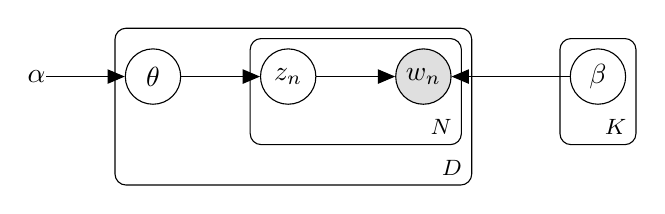
\begin{tikzpicture}
	  \node[latent] (z) {$z_n$} ; %
	  \node[obs, right = of z] (w) {$w_n$};
          \node[latent, left=of z] (theta) {$\theta$} ; %
          \node[const, left=of theta](alpha){$\alpha$};
          \node[latent, right=1.5 of w] (beta) {$\beta$};
        
          \edge {theta} {z} ; %
          \edge {z} {w} ;
          \edge {beta}{w} ;
          \edge {alpha}{theta}
          
          \plate {words}{
          	(z)
		(w)
	  }{$N$}
	  
          \plate {docs} {
          	(theta)
		(words)
          }{$D$}
          
          \plate {topicwords}{
          	(beta)
	 }{$K$}
    
	\end{tikzpicture}
	\end{figure}
\\The generative model describing the graphical representation:
	\begin{enumerate}
		\item For each document;
		\begin{enumerate}
			\item Topic proportions vector is drawn ($\theta \sim Dirichlet(\alpha)$)
			\item For each word in the document
			\begin{enumerate}
				\item A topic is drawn from topic proportions ($z_n \sim Multinomial(\theta)$)
				\item The word is drawn from topic ($w_n \sim Multinomial(\beta_{z_n})$)
			\end{enumerate}
		\end{enumerate}
	\end{enumerate}


\section{Posterior Probability}
When the \textit{topic-word} distributions are treated as fixed, the posterior distribution for $\theta$s and $z$s is:
\begin{equation}
P(\theta, z|w, \alpha, \beta) = \frac{P(\theta, z, w|\alpha, \beta)}{P(w|\alpha, \beta)}
\end{equation}
The joint distribution (for a single document) in the nominator is:
\begin{equation}
P(\theta, z, w|\alpha, \beta) = \frac{\Gamma(\sum_{i=1}^K \alpha_i)}{\prod_{i=1}^K\Gamma(\alpha_i)} \left(\prod_{i=1}^K \theta_i^{\alpha_i -1} \right) \left(\prod_{n=1}^N P(z_n|\theta)\prod_{j=1}^V\beta_{ij}^{[w_n = j]}\right)
\end{equation}
And the evidence (denominator) for a single document, can be written as:
\begin{equation}
P(w|\alpha, \beta) = \frac{\Gamma(\sum_{i=1}^K \alpha_i)}{\prod_{i=1}^K\Gamma(\alpha_i)} \int d\theta \left(\prod_{i=1}^K \theta_i^{\alpha_i -1} \right) \left(\prod_{n=1}^N\sum_{i=1}^K\prod_{j=1}^V(\theta_i\beta_{ij})^{[w_n = j]}\right)
\end{equation}
where $K$ is the number of topics in the corpus, $N$ is the number of words in the document and $V$ is the vocabulary size. Note that $P(z_n=i|\theta) = \theta_i$, and $P(w_n|\beta_i)$ is the discrete word distribution of topic $i$ over all words in the vocabulary.  We sum over all $z_n$s and integrate over $\theta$ to get the evidence. There are $K^N$ possible assignments to the words in a document, and we further take an integral over $\theta$, making the posterior intractable.

\section{Project Proposal}
In Gibbs Sampling, we are interested in the conditional distributions $P(\theta|z, w, \beta)$ and  $P(z_i|z_{\not{i}}, \theta, w, \beta)$ and they are given as:
\begin{align*}
P(\theta|z, w, \beta) = P(\theta|z) = & Dirichlet(\theta; \alpha + n(z_{1:K}))\\
P(z_i|z_{\not{i}}, \theta, w, \beta) = P(z_i|w_i, \theta) \propto P(z_i, w_i| \theta) =& P(z_i|\theta) P(w_i|\beta_{z_i})
\end{align*}
due to conditional independence properties of the model and the conjugacy of Dirichlet distribution to Multinomial. 

An iteration of the Gibbs Sampler is by sampling from the above distributions, repeatedly in turn. 

We can also integrate out $\theta$ and sample $z_i|z_{\not{i}}, w, \beta$s. $P(z_i|z_{\not{i}}, w, \beta)$ is given as:
\begin{align*}
P(z_i|z_{\not{i}}, w, \beta) = \int d\theta P(z_i, \theta|w_i) \propto \int d\theta P(z_i, w_i, \theta) =& \int d\theta P(\theta) P(z_i|\theta) P(w_i|\beta_{z_i})\\
=&n_{z_i}(z_{\not{i}})P(w_i|\beta_{z_i})
\end{align*}
where $n_{z_i}(z_{\not{i}}) = \sum_{i^\prime \neq i}[z_{i^\prime} = z_i]$, number of assignments (in the current iteration) to the \textit{same topic} as $z_i$ of \textit{other words}, giving the Collapsed Gibbs Sampling update rule.

$\beta$s can also be treated as Dirichlet random variables. In this case the conditional word distribution for each topic $k$, $\beta_{kj}$ given the others is again a Dirichlet, depending only on the number of words assigned to topic $k$ and the number of times the word $j$ is assigned to the topic. It is also possible to sample from $z_i|z_{\not{i}}, w$ in the collapsed version, which we do not show here.

As the project, we are going to implement either the usual Gibbs Sampler, or the collapsed version, and report experiments on a dataset. Mixed Membership Models are more general than the topic modeling task, as an example, another use case is for Collaborative Filtering using individuals' interactions with items---as an analogy, here, an entire user history corresponds to a document. We have not decided on the experimental dataset yet, but it is likely to be from one of these two domains.
% that's all folks
\end{document}


